\documentclass[dvips]{article}
\usepackage{makeidx}
\usepackage[dvips]{graphicx}
\usepackage[dvips]{changebar}
\usepackage{html,htmllist}
% \usepackage{times}
\scrollmode
% use %sort -f -u manual.idx > manual.index for a primitive index
%
%  NOTE:  You must use LaTeX2e in order to process this document
%	If you do not have LaTeX2e, a PostScript version
%	(manual.ps) is included with this distribution.
%
%%%%%%%%%%%%%%%%%%% No changes beyond this point %%%%%%%%%%%%%%%%%%%%%%%%%%%%%

\makeindex
\sloppy
% Transforms the \indexentry generated by \makeindex in the concepts.idx
% file into a form understood by the theindex environment.
% See below on how to produce an index.
%
\newcommand{\latextohtml}{\LaTeX 2\texttt{HTML}}
\newcommand{\fn}[1]{{\ttfamily #1}}	% file names
\newcommand{\Email}[1]{{\ttfamily <#1>}}% file names
\newcommand{\HTML}[1]{{\ttfamily <#1>}}%  HTML tag
\newcommand{\Meta}[1]{\texttt{<\emph{#1}>}}%  Meta string
\newcommand{\indexentry}[2]{\item #1 #2}
\newcommand{\onlinedoc}{http://www-dsed.llnl.gov/files/programs/unix/latex2html/manual/}
\newcommand{\patches}{http://www-dsed.llnl.gov/files/programs/unix/latex2html}
\newcommand{\sourceA}{ftp://www-dsed.llnl.gov/files/programs/unix/latex2html/sources/latex2html-96.1.tar.gz}
\newcommand{\sourceB}{ftp://ftp.mpn.com/pub/nikos/latex2html-96.1.tar.gz}
\newcommand{\sourceC}{ftp://ftp.rzg.mpg.de/outgoing/latex2html-96.1.tar.gz}
\newcommand{\CTAN}{tex-archive/support/latex2html}

\setlength{\textwidth}{5.5in}
\setlength{\changebarwidth}{1pt}
\addtolength{\oddsidemargin}{-1in}
\addtolength{\evensidemargin}{-1in}
\begin{document}
\sloppy
\title{The \latextohtml{} Translator}
\author{Nikos Drakos,\\ Computer Based Learning Unit,\\ University of
Leeds.}
\date{\today}
\maketitle 

\centerline{\large This document accompanies \latextohtml{}
Version 96.1\footnote{This manuscript was updated to version 96.1
as indicated by the changebars by Herbert W.\ Swan
\Email{dprhws@edp.Arco.com} and converted to \LaTeXe{} by Michel
Goossens \Email{goossens@cern.ch}.}}

\begin{htmlonly}
A \htmladdnormallink{postscript version}{manual.ps}
is available. \index{postscript version}

\textbf{Warning:} The contents of this document are likely to change.
It is advisable not to use links to any pages other than the first
page (this page).
\end{htmlonly}

\begin{abstract} 
\latextohtml{} is a conversion tool that allows documents
written in \LaTeX\  to become part of the WorldWide Web.
In addition, it offers an easy migration path towards
authoring complex hypermedia documents using
familiar word-processing concepts.

\latextohtml{} replicates the basic structure of a \LaTeX\  document 
as a set of interconnected HTML files which can be explored using
automatically generated navigation panels. 
The cross-references, citations, footnotes, the table of contents and the lists
of figures and tables, are also translated into hypertext links. Formatting
information which has equivalent ``tags'' in HTML (lists, quotes, paragraph
breaks, type styles, etc.) is also converted appropriately. 
The remaining heavily formatted items
such as mathematical equations, pictures or tables are converted to images
which are placed automatically at the correct positions in the
final HTML document.

\latextohtml{} extends \LaTeX\  by supporting arbitrary hypertext links 
and symbolic cross-references between evolving 
remote documents. It also allows the specification
of \emph{conditional text} and the inclusion of raw HTML commands.
These hypermedia extensions to \LaTeX\  are available as 
new commands and environments from within a \LaTeX\  document.

This document presents the main features of \latextohtml{}, and
describes how to obtain, install, and use it.
\end{abstract}

\pagebreak
\tableofcontents
\listoffigures
\listoftables

\pagebreak

\section{Overview}
\index{overview}
This document describes the \latextohtml{} translator which:

\begin{itemize}
\item breaks up a document into one or more components as specified
by the user\footnote{The user can specify the \emph{depth} at which 
the document should not be broken up any further.},
\item provides optional, customizable iconic navigation
panels on every page which contain links to other parts of the
document, or other documents,
\index{inlined equations}
\item hadles inlined equations ( \(\sum_{i=1}^{n} x_{i} =
\int_{0}^{1} f \)), handles equation alignment ($A_{B_{C+D}}$), 
right-justified numbered equations
(see equation \ref{eq:demo}), tables (see Table \ref{tab}), or
figures (see Figure \ref{fig:example}),
and \emph{any arbitrary environment}\footnote{These are
passed to \LaTeX\  and then converted to images which are either included
in the document or are made available through hypertext links.},
\item 
\begin{changebar}
figures or tables can be arbitrarily scaled 
and oriented and shown either as inlined images or ``thumbnail'' sketches
\end{changebar}
\item can produce output suitable for browsers that support inlined
images or character based browsers (as specified by the user),
\item handles definitions of new commands, environments, and theorems
even when these are defined in external style files\footnote{
This allows the definition of HTML macros in \LaTeX\   !},
\item handles footnotes\footnote{Like this!}, tables of contents, lists
of figures and tables, bibliographies, and can generate an
\index{index} index,
\item translates cross-references into hyperlinks and 
extends the \LaTeX\  cross-referencing mechanism to work
not just within a document but \emph{between documents} which may
reside in remote locations, \index{ISO-LATIN-1}
\item translates \LaTeX\  accent and special character commands
(e.g. \. {A} \O \"o \pounds \copyright \P) to
the equivalent ISO-LATIN-1 or Unicode character set where possible,
\item recognizes hypertext links (to multimedia resources or
arbitrary internet services such as sound/video/ftp/http/news) and
links which invoke arbitrary program scripts,
all expressed as \LaTeX\  commands,
\item recognizes \emph{conditional text}  which is intended only for
the hypertext version, or only for the paper (DVI) version,
\item can include raw HTML in a \LaTeX\  document (e.g. in order to
specify interactive forms),
\item can deal sensibly at least with the \emph{Common \LaTeX\   commands}
summarized at the back of the \LaTeX\   blue book \cite{lamp:latex},
\item will try and translate any document with embedded \LaTeX\  commands 
irrespective of whether it is complete or syntactically legal.
\begin{changebar}
\item 
can be configured to translate equations and/or tables either
as GIF images or as HTML 2.1 or 3.0 markup, as browsers become available
which are suitable for the task.
\item links symbolic references across document segments which are
independently processed.
\end{changebar}
\end{itemize}

A selection of documents illustrating the different contexts in 
which \latextohtml{} has been used is available at \\
\htmladdnormallink{\onlinedoc}{\onlinedoc}.

\section{User Manual}
\index{man page} \label{sec:man}

To use \latextohtml{} simply type \fn{latex2html <file>.tex}.
\begin{changebar} The \fn{.tex} suffix is optional and will be supplied
by the program if it is omitted by the user. \end{changebar}
This will create a new directory called \texttt{file} which will contain 
the generated HTML files, some log files and possibly some images.
To view the result use an HTML viewer such as \htmladdnormallink{NCSA 
Mosaic}{http://www.ncsa.uiuc.edu/SDG/Software/Mosaic/Docs/help-about.html}
or \htmladdnormallink{Netscape Navigator}{http://home.netscape.com}
on the main HTML file which is \fn{file/file.html}. This file will
contain navigation links to the other parts of the generated document.

It is possible to customize the output from \latextohtml{} using a number
of \hyperref{command line options}{command line options (see Section
}{)}{options}
with which you can specify how to break up the document, where to put 
the generated files, what the title is, what the signature at the end
of each page is, what to put in the navigation panel, what kind of
extra information to include about the document, whether to retain
the original \LaTeX\  section numbering scheme, etc.

Also, the \latextohtml{} script includes a short manual which can be 
viewed by saying \verb|%nroff -man latex2html|.

\subsection{Command Line Options}
\index{options}\label{options}
The command line options described below can be used to change the
default behavior of \latextohtml. Alternatively, the corresponding 
environment variables
in the initialization file \fn{.latex2html-init} may be changed, in
order to achieve the same result.

\begin{htmllist}
\label{listExample}
\htmlitemmark{PurpleBall}
\item [-split \textsl{num}]
Stop splitting sections into separate files at this depth.
A value of 0 will put the document into a 
single HTML
file. The default is 8.
\item [-link \textsl{num}]
Stop revealing child nodes at each node at this depth. 
(A node is a part/chapter/section/subsection/subsubsection etc.).
A value of 0 will show no links to child nodes, a value of 1 
will show only the immediate descendents, etc. A value
at least as big as that of the \texttt{-split}
option will produce a table of contents for
the tree structure, rooted at each given node. The default is 4.
\label{page:nolatex}
\item [-nolatex ]
Disable the mechanism for passing unknown environments to \LaTeX\ for processing.
This can be thought of as ``draft mode'' which allows  faster translation of the 
basic document structure and text, without fancy figures, equations or
tables. 

\textbf{This option has been superceded by the \texttt{-no\_images} option
(see below)}.
\item [-external$\_$images]
Instead of including any generated images inside the document, leave them
outside the document and provide hypertext links to them.
\label{asciimode} 
\item [-ascii$\_$mode]
Use only ascii characters and do not include any images in the final output.
In ascii mode the output of the translator can be used on
character based browsers which do not support inlined images (the \HTML{IMG} tag).
\item [-t \textsl{top-page-title}]
Name the document using this title.
\item [-up\_url \textsl{URL}] 
\begin{changebar}
Specifies a universal resource locator (URL) to associate
with the UP button of the top-level navigation panel.
\item [-up\_title \textsl{string}] Specifies a title associated with this URL.
\item [-down\_url \textsl{URL}]
Specifies a URL for the NEXT button of the bottom-level navigation panel.
\item [-down\_title \textsl{string}] Specifies a title associated with this URL.
\item [-contents \textsl{URL}] Specifies a URL for the table of contents button
for document segments that would not otherwise have one.
\item [-index \textsl{URL}] Specifies a URL for the index button for document segments
that otherwise would not have an index.
\item [-external\_file \textsl{filename-prefix}]  Specifies the prefix of the
\texttt{.aux} file that this document segment should read.  The 
\texttt{.aux} extension will be appended to this prefix.  This file
is necessary for document segments to obtain figure and section
numbers from \LaTeX.
\end{changebar}
\item [-dir \textsl{output-directory}]
Redirect the output to this directory. 
\item [-no\_subdir]
Place the generated HTML files  in the 
current directory. The default behaviour is to create (or reuse)
another file directory.
\begin{changebar}
\label{prefix}
\item [-prefix \textsl{filename-prefix}]
  The \texttt{filename-prefix}\index{filename prefix}
  will be prepended to all \texttt{.gif, .pl}
  and \texttt{.html} files produced, except for the top-level \texttt{.html}
  file.  This will enable multiple products of \latextohtml{} to
  peacefully coexist in the same directory.  Do \textbf{not}, however,
  attempt to \emph{simultaneously} run multiple instances of
  \latextohtml{} using the same output directory, or various temporary
  files will overwrite each other.
\item [-font\_size \textsl{size}]
  This option provides better control over the font size of environments
  processed by \LaTeX.  \textsl{size} must be one of the font sizes
  that \LaTeX\ recognized; i.e.\ \fn{10pt, 11pt, 12pt}, etc.  The
  default size is the same as the \LaTeX\ document.  Whatever size is
  selected, it will be magnified by the installation variables,
  \$MATH\_SCALE\_FACTOR or \$FIGURE\_SCALE\_FACTOR.
\item [-no\_tex\_defs]
  If specified, the translator will make no attempt to interpret
  raw \TeX\ commands.  This feature will enable sophisticated authors
  the ability to insert arbitrary \TeX\ commands in environments
  that are distined to be processed by \LaTeX\ anyway (e.g.\ figures,
  theorems, etc.)
\end{changebar}
\item [-ps\_images]
Use links to external postscript images rather than inlined GIF images.
\item [-address \textsl{author-address}]
Sign each page with this address. \label{navoptions} 
\item [-no$\_$navigation]
Disable the mechanism for putting navigation links in 
each page.
\item [-top$\_$navigation]
Put navigation links 
at the top of each page.    
\item [-bottom$\_$navigation]
Put navigation links 
at the bottom of each page AS WELL as the top.
\item [-auto$\_$navigation]
Put navigation links
at the top of each page. If the page exceeds \verb|$WORDS_IN_PAGE| number of words
(the default is 450) then put one at the bottom of the page as well.
\item [-index$\_$in$\_$navigation]
Put a link to the index page in the navigation panel if there is an index.
\item [-contents$\_$in$\_$navigation]
Put a link to the table of contents in the navigation panel if there is a 
table of contents.
\item [-next\_page\_in\_navigation]
Put a link to the next logical page in the navigation panel.
\item [-previous\_page\_in\_navigation]
Put a link to the previous logical page in the navigation panel.
\item [-info \textsl{string}]
Generate a new section \emph{About this document ...} containing information
about the document being translated. The default is to generate such a section 
with information on the original document, the date, the user and the
translator.
An empty string (or the value 0) disables the creation of this extra
section. If a non-empty string is given, it will be placed in the contents of the 
\emph{About this document ...} section instead of the default information.
\item [-reuse \textsl{reuse\_option}]
\begin{changebar} 
The \textsl{reuse\_option} specifies how or whether image files are to be shared
or recycled, and accepts three valid options:
\begin{htmllist}
\item [0] Do not ever share or recycle image files. This choice also invokes an
	interactive session prompting the user about what to do about
	a pre-existing \texttt{HTML} directory, if it exists.
\item [1] Recycle image files from a previous run if they are available,
	but do not share identical images that must be created in this run.
\item [2] Recycle image files from a previous run and share identical
	images from this run.  (This is the default).
\end{htmllist}
Section \ref{recycling} provides additional information about image reuse.
\item [-no\_reuse]
Do \textbf{not} share or recycle images generated during previous translations.
This is equivalent to \textbf{-reuse 0}.
(This will enable the initial interactive session during which the user is
asked whether to reuse the old directory, delete its contents or quit)
\end{changebar}
\item [-init\_file file]
Load the specified file. This Perl file will be loaded after loading 
\$HOME/.latex2html-init (if one exists). It can be used to change the 
default options.
\item [ -no\_images]
Do not attempt to produce any inlined images. 
The missing images can be generated "off-line" by restarting \latextohtml{}
with the option \texttt{-images\_only}.
\item [ -images\_only]
Try and convert any inlined images that were left over from previous
runs of \latextohtml. 
\item [ -show$\_$section$\_$numbers]
Show section numbers. By default the section numbers are not shown 
in order to encourage the 
use of particular sections as standalone documents. 
In order to be shown, section titles must be unique and must not
contain inlined graphics.
\item [ -html\_version \textsl{version}]
This specifies the \texttt{HTML} \htmlref{version}{versions}
\index{HTML versions}
to generate.  Currently, versions 2.1, 2.2, 3.0 and 3.1 are
available.  The default version is 2.0.
\begin{changebar}
\item [ -vs] Print the current version of \latextohtml.
\end{changebar}
\item [-h]
Print out the list of options.
\end{htmllist}

\subsection{Extending the Translator}
\label{sec:extend}
As the translator covers only partially the set of \LaTeX\  commands
and
because new \LaTeX\  commands can be defined arbitrarily using low level 
TeX commands, the translator should be flexible enough to allow end
users
to specify how they want particular commands to be translated. 

\subsubsection{Adding Support for Specific Style Files}
\label{sec:sty}
\latextohtml{} provides a mechanism where code to translate specific
style files is automatically loaded if such code is available.
When the use of a style
file such as \fn{german.sty} is detected in a \LaTeX\  source
document,
the translator looks for a file \fn{LATEX2HTMLDIR/styles/german.perl}.
If one is found, then it will be loaded into the main script. 

This mechanism will help to keep the core script smaller as well as make
it easier for others to contribute and share solutions on  
how to translate specific style files.
\begin{changebar}
The current distribution includes the files listed in Table \ref{styles}.
These will provide
good examples of how you can create your own extensions to \latextohtml.
\end{changebar}
\begin{table}
\begin{center}
\begin{tabular}{|c|p{3in}|}
\hline
\fn{.perl} file & \centerline{Description} \\
\hline
\fn{alltt} & Supports the \LaTeXe's \fn{alltt} package \\
\fn{changebar} & Provides rudimentary change bar support \\
\fn{color} & Causes colored text to be processed as ordinary text by \latextohtml \\
\fn{french} & Special support for the French language \\
\fn{epsfig} & Processes embedded figures not enclosed in a \fn{figure} environment \\
\fn{floatfig} & Processes floating figures \\
\fn{german} & Special support for the German language \\
\fn{graphics} & Supports commands in the \fn{graphics} package \\
\fn{graphicx} & Supports the alternate syntax of graphics commands \\
\fn{heqn} & Alters the way displayed equations are processed  \\
\fn{htmllist} & Provides support for fancy lists \\
\fn{makeidx} & Generates indices \\
\fn{texdefs} & Supports raw \TeX\ commands \\
\fn{wrapfig} & Supports wrapped figures \\
\hline
\end{tabular}
\end{center}
\caption{Supported \latextohtml\ style files\label{styles}}
\end{table}
The problem however, is that writing such extensions requires an understanding 
of Perl and of the way \latextohtml{} is organized. More user-friendly 
interfaces will be  investigated.

At the moment a rudimentary mechanism is provided so that 
a user can ask for particular commands and their arguments either to be
ignored or passed on to \LaTeX\  for processing (the default behavior
for unrecognized commands is for their arguments to remain in the HTML
text).
Commands that are passed on to \LaTeX\  are converted to images which
are either ``inlined'' in the main document or become accessible via
hypertext links.
Simple extensions using the commands above may be included in the 
\fn{LATEX2HTMLDIR/latextohtml.config} file or in each personal 
\fn{HOME/.latex2html-init} initialization file.

\subsubsection{Asking the Translator to Ignore Commands}
Commands that should be ignored may be specified in the 
\fn{.latex2html-init}
file as input to the \verb|ignore_commands| subroutine. 
Each command which is to be ignored should be on a separate line 
followed by compulsory or optional argument markers separated by 
{\verb|#|}'s e.g.\footnote{It is possible to add arbitrary Perl code
between any of the argument markers which will be executed when 
the command is processed. For this however a basic understanding of
how the translator works and of course Perl is required.}:
\begin{verbatim}
<cmd_name>#{}# []# {}# [] ...
\end{verbatim} 
\verb|{}|'s mark compulsory arguments and \verb|[]|'s optional ones.

Some commands may have arguments which should be left as text even
though the command should be ignored (e.g. \texttt{mbox},
\texttt{center}, etc.). In these cases the arguments should be left
unspecified.

Here is an example of how this mechanism may be used:
\begin{verbatim}
&ignore_commands( <<_IGNORED_CMDS_);
documentstyle # [] # {}
linebreak# []
center
<add your commands here>
_IGNORED_CMDS_
\end{verbatim}
\subsubsection{Asking the Translator to Pass Commands to \LaTeX}
\label{pass}
Commands that should be passed on to \LaTeX\  for processing because
there is no direct translation to HTML may be specified in the 
\fn{.latex2html-init}
file as input to the \verb|process_commands_in_tex|
subroutine.
The format is the same as that for specifying commands to be ignored.
Here is an example:
\begin{verbatim}
&process_commands_in_tex (<<_RAW_ARG_CMDS_);
fbox # {}
framebox # [] # [] # {}
<add your commands here>
_RAW_ARG_CMDS_
\end{verbatim}

\section{Hypertext Extensions to \LaTeX}
\label{special} \index{hypertext extensions}
\begin{changebar}
This section describes how you can define hypertext entries in
your \texttt{HTML} documents from within your \LaTeX\ source.
\end{changebar}
These are implemented as new \LaTeX\ commands which have special 
meaning during the translation to \texttt{HTML} but are mostly ignored when
processed by \LaTeX.

\index{html style file}
All the new commands used in the sections 
below are defined in the file \htmladdnormallink{\fn{html.sty}},
which is part of the 
distribution. \emph{This file must be included in any 
\LaTeX\ document using these features} by one of the following methods:

\begin{changebar}
\begin{itemize}
\item Including \fn{html} as an optional argument to the \LaTeX\ 
\texttt{documentstyle} command;
\item Including \fn{html} in the \LaTeXe{} \texttt{usepackage} command; or
\item Pasting the definitions of individual commands
directly into the text!
\end{itemize}
\end{changebar}

\subsection{Hyperlinks in \LaTeX}
\label{sec:hyper} \index{hyperlinks} \index{htmladdnormallink} \index{htmladdimg}
Arbitrary hypertext references are available 
through the commands 
\texttt{htmladdnormallink} and \texttt{htmladdimg}.

These are defined as follows:
\begin{verbatim}
\htmladdnormallink{<text>}{<URL>}
\htmladdimg{<URL>}
\end{verbatim}
The first command expects some text as the first argument and a URL as
the second argument. When processed by \LaTeX\  (i.e. in the \texttt{dvi }
or \texttt{ps} output files), the URL will have no effect.
But when processed by the 
translator, 
\htmladdnormallink{the URL will be used to provide
an active hypertext link}
{http://www.ncsa.uiuc.edu/demoweb/url-primer.html} (to another
file, picture, sound file, movie, etc) e.g.
\begin{verbatim}
\htmladdnormallink{<URL>}
	{http://www.ncsa.uiuc.edu/demoweb/url-primer.html}
\end{verbatim}

A similar command called \texttt{htmladdnormallinkfoot} 
takes the same two arguments and has the same effect when generating
HTML as \texttt{htmladdnormallink}. But when processed by \LaTeX\  it shows
the 
URL as a footnote.

In a similar way, the argument of the \texttt{htmladdimg} command 
should be a URL pointing to an image.  This URL is ignored in
the \LaTeX\  hard copy output. 

\subsection{Including Arbitrary HTML Markup}
\index{HTML+} 
Raw HTML or HTML+ tags and text may be included using the environment 
\texttt{rawhtml}. This can be used to take advantage
of new HTML+ facilities as soon as they become available.
\index{electronic forms} A particularly
good use of this feature is in the creation of interactive
\htmladdnormallink{electronic forms}{http://south.ncsa.uiuc.edu/forms.html}
from within a \LaTeX\  document. When producing the paper (DVI) version
of a document the \texttt{rawhtml} environment is ignored.

Here is an example: \index{rawhtml}
\begin{small}
\begin{verbatim}
\begin{rawhtml}
<HR>
<FORM ACTION="http://cbl.leeds.ac.uk/nikos/doc/error.html">
<OL>
<LI> <INPUT TYPE="checkbox" NAME="wp" VALUE="word"> Word for
Windows.
<LI> <INPUT TYPE="checkbox" NAME="wp" VALUE="wp"> Word Perfect.
\end{verbatim}
\begin{verbatim}
<LI> <INPUT TYPE="checkbox" NAME="wp" VALUE="latex"> LaTeX.
<LI> Plain Text Editors (Please Specify): <INPUT TYPE="text" NAME="other_ed">
</OL>
So, what do think (comments please): <BR>
<INPUT TYPE="text" SIZE=45,4 NAME="other_wp">

<INPUT TYPE="submit" VALUE="submit this form but don't expect much!">
</FORM>
<HR>
\end{rawhtml}
\end{verbatim}
\end{small}
\begin{rawhtml}
The result is shown below. 
<HR>
<FORM ACTION="http://cbl.leeds.ac.uk/nikos/doc/error.html">
<OL>
<LI> <INPUT TYPE="checkbox" NAME="wp" VALUE="word"> Word for
Windows.
<LI> <INPUT TYPE="checkbox" NAME="wp" VALUE="wp"> Word Perfect.
<LI> <INPUT TYPE="checkbox" NAME="wp" VALUE="latex"> LaTeX.
<LI> Plain Text Editors (Please Specify): <INPUT TYPE="text" NAME="other_ed">
</OL>
So, what do think (comments please): <BR>
<INPUT TYPE="text" SIZE=45,4 NAME="other_wp">

<INPUT TYPE="submit" VALUE="submit this form but don't expect much!">
</FORM>
<HR>
\end{rawhtml}

\begin{latexonly}
The result is shown below:
\begin{figure}
    \begin{center}
    \fbox{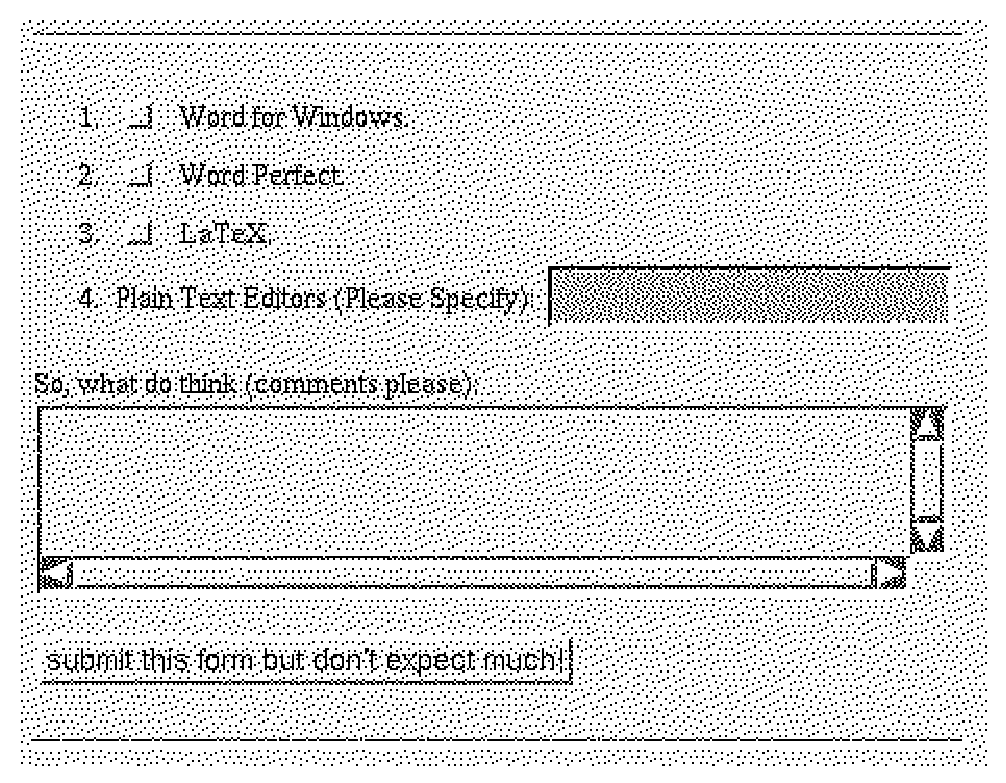
\includegraphics[width=4in]{eform.ps}}
    \end{center}
    \caption{An electronic form. Of course in the online version of this
     document the form above would be active.}
\end{figure}
\end{latexonly}

\textbf{Warning:} Avoid using \LaTeX\  commands involving counters (e.g.
numbered figures or equations) in conditional text because this may 
disrupt the values of the counters in the electronic version.

% The argument here used to have a \label in its argument which caused
% the ``Contents'' page entry not to be hyperized.
\subsection{Conditional Text}
\label{sec:latexonly}
\index{latexonly} \index{htmlonly} Conditional text can be specified
using the environments \texttt{latexonly} and \texttt{htmlonly}. These
allow writing parts of a document which are intended only for
electronic delivery or only for paper-based delivery.

This would be useful for example in adding a long description of a
multimedia resource in the paper version of a document. Such a
description would be redundant in the electronic version, as the user
can have direct access to this resource. 

Here is an example of the use of the \texttt{latexonly} environment:

\begin{verbatim}
\begin{latexonly}
\begin{figure}
    \begin{center}
    \fbox{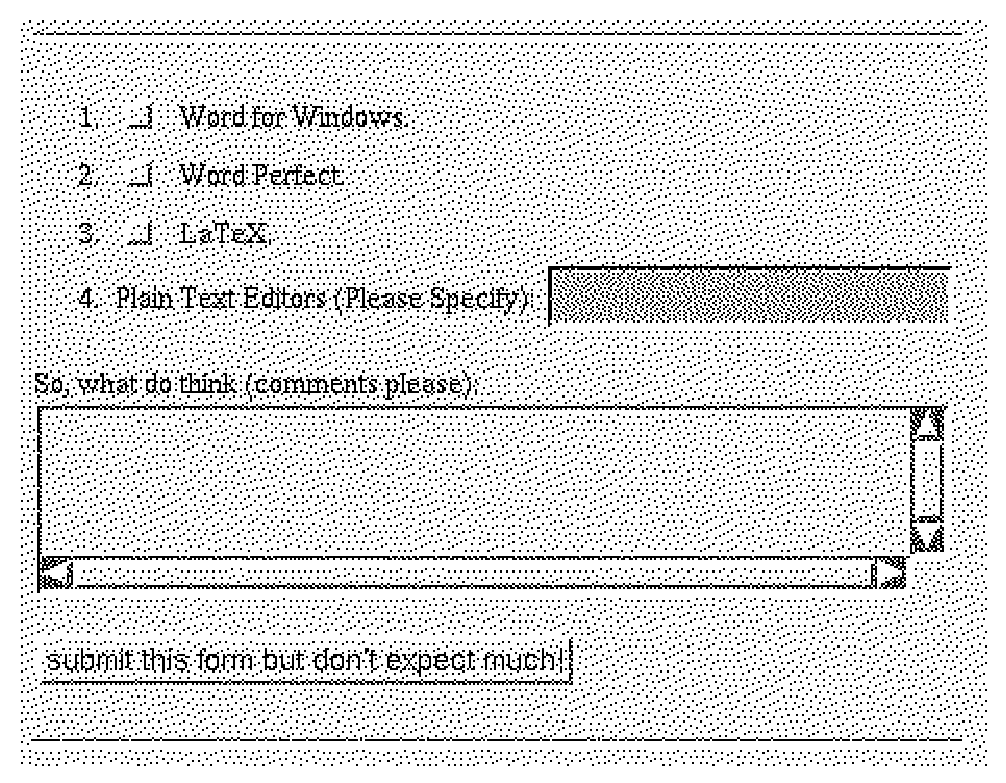
\includegraphics[width=4in]{eform.ps}}
    \end{center}
    \caption{An electronic form. Of course in the online version of this
     document the form above would be active.}
\end{figure}
\end{latexonly}
\end{verbatim} 

\begin{changebar}
There are also shorthand notations to accomplish the same thing
with less typing.  The \verb|\latex{}| command causes everything
within the braces to be processed by \LaTeX, but ingored by
\latextohtml.  Conversely, the \verb|\html{}| command causes
everything within the braces to be ignored by \LaTeX\ and
processed by \latextohtml.  Finally the command
\verb|\latexhtml{}{}| causes everthing within the first set
of braces to be processed exclusively by \LaTeX, with
the contents of the second set of braces processed solely
by \latextohtml.
\end{changebar}

\subsection{Symbolic References Shown as ``Hyperized'' Text}
\label{hyperized}
\index{cross-references}
In printed documents cross-references are shown through a \emph{numerical
or symbolic indirection} e.g. ``see Figure 1'' (numeric indirection), or
``see section ``Changes'' (symbolic indirection).  \latextohtml{} can
mirror this mechanism using the same numeric or symbolic references,
or when these are
not appropriate by using iconic references.

In a hypertext document however, cross-references can be shown 
without any indirection just by highlighting a relevant piece of
text. This can make a document more readable as it removes unnecessary
information. 

A single new \LaTeX\  command \texttt{hyperref} can be used for
specifying how a cross-reference should appear both in the printed
document and in the hypertext version.

Assuming that the label \verb|sec:cond| is defined somewhere
in a document the command \texttt{hyperref} which takes 4 arguments
can be used in the same document as follows:

\index{hyperref} \index{conditional text}
\begin{verbatim}
\emph{Is the concept of
\hyperref
% This will be highlighted in the hypertext version
{conditional text}			% argument #1
% This will be shown in the printed version 
% followed by a numeric reference ...      
{conditional text (see Section }  	% argument #2
% ... followed by this text
{ for more information)} 		% argument #3
% This the common label 
{sec:cond}				% argument #4
a good idea? }
\end{verbatim}

Here is how it will be shown: \\
{Is the concept of
\hyperref
% This will be highlighted in the hypertext version
{conditional text}
% This will be shown in the printed version  
% followed by a numeric reference ...      
{conditional text (see Section }  
% ... followed by this text
{ for more information)} 
% This the common label 
{sec:cond}
a good idea? }

\begin{htmlonly}
In the printed version what would appear is: \\
{ Is the concept of conditional text (see Section XXX for more information) a good idea? }
\end{htmlonly}

\begin{latexonly}
In the hypertext version what would appear is:\\
{ Is the concept of \underline{conditional text} a good idea?} \\
Of course \underline{conditional text} would be an active hypertext link.
\end{latexonly}


Another command also defined in \fn{html.sty} is \texttt{htmlref} 
which has the same effect as \texttt{hyperref} during the conversion to
HTML.
It takes two arguments, some text and a label. In the HTML version the
text will be ``hyperized'' pointing to the label. In the paper version
the text will be shown as it is and the label will be ignored eg

\begin{small}
\begin{verbatim}
With \texttt{htmlref} \htmlref{it's easy to make links}{fig:example}.
\end{verbatim}
\end{small}

\begin{htmlonly}
In the HTML version it will be shown as: \\
With \texttt{htmlref} \htmlref{it's easy to make links}{fig:example}.
\end{htmlonly}
\begin{latexonly}
In the HTML version it will be shown as: \\
With \texttt{htmlref} \underline{it's easy to make links}.
\end{latexonly}
\subsection{Symbolic References Between Living Documents}
\label{external_cross}
\begin{changebar}
The method of the previous section to generated
symbolic \htmlref{hyperized}{hyperized} links can
easily be extended to \emph{external} documents
processed by \latextohtml.  When \latextohtml{}
processes a document, it generates a \texttt{perl} file named \fn{labels.pl}
\index{labels.pl}
which contains a list of all the symbolic labels that were defined, along with
their locations.  The name of this file is preceeded by
the \htmlref{filename prefix}, to allow different document segments
to share the same directory.  Links to an external
document are then possible once a connection is established
to that document's \fn{labels.pl} file.  This connection is
established by the \verb|\externallabels| command:
\index{externallabels}\index{externalref}
\end{changebar}

\begin{verbatim}
\externallabels{<URL to directory of external document>}
               {<external document labels.pl file>}
\end{verbatim}

The first argument to \fn{externallabels} should be a URL to 
the directory containing the external document.  
The second argument
should be the full pathname to the \fn{labels.pl} file belonging
to the external document.  Note that for \emph{remote} external documents
it is necessary to copy the \fn{labels.pl} file locally so that it
can be read when processing a local document that uses it.
The command \texttt{externallabels} can be used once for each external
document in order to import the 
\textit{external labels}\label{externallabels}\index{labels, external}
into the current document.
A warning is given if \fn{labels.pl} cannot be found.

\begin{changebar}
If a symbolic reference made in either of the commands described in
Section \ref{hyperized} is not defined within the document itself,
\latextohtml{} will look for that reference in one of the external
files.\footnote{Care must be taken to ensure that critical symbolic
references are unique across related documents.}
After any modifications in an external document (sections added/deleted,
segmentation into different physical parts, etc.) a new \fn{labels.pl}
will be generated.  If the \texttt{externallabels} command in another 
document contains the correct address
to the \texttt{labels.pl} file, then the cross-references will be realigned
after running the local document through the translator.

There is also a mechanism analogous to the
\texttt{label-ref} pairs of \LaTeX, which can be used only 
within a single document. These labels are called
\textit{internal labels}\label{internallabels}\index{labels, internal},
as opposed to the \htmlref{external labels}{externallabels} defined above.

Either type of label is defined with a \LaTeX\ 
\texttt{label} command.  Labels can be referenced \textit{within}
a document using a \texttt{ref} command.
When processed by \LaTeX, each \texttt{ref} command is replaced by the 
section number in which the corresponding \texttt{label} occurred.
When processed by the translator, each \texttt{ref} is replaced by 
a hypertext link to the place where the corresponding \texttt{label}
occurred.  This mechanism can be extended to external documents
by the \verb|\externalref{}| command:

\begin{verbatim}
\externalref{<symbolic label in remote document>}
\end{verbatim}

The argument to \texttt{externalref} may be any symbolic label defined 
in any of the external documents in the same
Such references to external symbolic labels are then translated
into hyperlinks pointing to the external document.
\end{changebar}

\subsubsection{A Cross-referencing example}
\label{crossrefs} 
To understand this mechanism better consider 
how you would maintain a link to this section  
(of the hypertext version of this document) from one of your documents
without using labels.
Sure enough you can get the
name of the physical file that this section is in. This however is very
likely to change and any links to it will become invalid. To update 
your link, the name of the new file must be found and your link changed 
by hand. Also there is no general updating mechanism so the only way to
find
out if your document is pointing to the right place is by actually
following the link and then doing a manual update\footnote{
Link validation can be done automatically but the updating must be
done
manually when filenames have changed (assuming no other symbolic label
mechanism is available).}.

Now consider how it could be done with symbolic labels. 
First you have to import the labels used in this document 
by copying the file 
\htmladdnormallink{labels.pl}
{http://cbl.leeds.ac.uk/nikos/tex2html/doc/manual/labels.pl},
saving it say
in \texttt{/tmp/labels.pl},
and then adding anywhere in your document:
\begin{verbatim}
\externallabels{http://cbl.leeds.ac.uk/nikos/tex2html/doc/manual}
               {/tmp/labels.pl}
\end{verbatim}
After that you can use the label \texttt{crossrefs} defined at the beginning of this 
section\footnote{You either have to guess the role of each label by
looking at the \texttt{labels.pl} file or by asking the author!} as follows:
\begin{verbatim}
\externalref{crossref}
\end{verbatim}
This will be translated into the appropriate hyperlink to this page.
If there are any changes in this document and you would like to
bring your document upto date you have to copy 
\htmladdnormallink{labels.pl}
{http://cbl.leeds.ac.uk/nikos/tex2html/doc/manual/labels.pl} again
and rerun the translator on your document. Of course if I move the 
directory containing the HTML files for this document somewhere else 
then you would have to make a change in the argument of the 
\texttt{externallabels} command to reflect this. 

It is obvious that some level of collaboration is required between
authors trying to maintain cross-references between different documents. 
Using symbolic labels makes this a lot easier (especially for documents
written by the same author).

\subsection{Document Segmentation\protect\footnote{This feature
is supported only for users of \LaTeXe.}\label{Segmentation}}
\begin{changebar}
One of the greatest appeals of the World Wide Web is its high
connectivity through hyperlinks.  As we have seen, the \LaTeX\ 
author can provide these links either manually or symbolically.
Manual links are more tedious because a URL must be provided
by the author for every link, and updated every time the target
documents change.
Symbolic links are more convenient, because the translator
keeps track of the URLs.  Earlier releases of \latextohtml\ 
required the entire document to be processed together if it
was to be linked symbolically.  However, it was easy for
large documents to overwhelm the memory capacities of moderate
sized computers.  Furthermore, processing time could become
prohibitively high, if even a small change required the
entire document to be reprocessed.

For these reasons, program segmentation was developed.
This feature enables the author to subdivide his document
into multiple \textit{segments}\label{segments}\index{program segments}.
Each segment can be processed independently by \latextohtml.
Hypertext links between segments can be made symbolically,
with references shared through
auxiliary files.  If a single segment changes, only that
segment needs to be reprocessed (unless a label is changed
that another segment requires).  Furthermore, the entire
document can be processed without modification by \LaTeX\ 
to obtain the printed version.  The top level segment
that \LaTeX\ reads is called the \emph{parent} segment.  The
others are called \emph{child} segments.

Program segmentation does require a little more work on the
part of the author, who will now have to untertake some
of bookkeeping formerly performed exclusively by \latextohtml.
The following four \LaTeX\ extensions carry out segmentation:
\begin{htmllist}
\htmlitemmark{BlueBall}
\item \verb|\segment{file}{sec-type}{heading}|
This commands indicates the start of a new program segment.
This segment resides in \fn{file.tex}, represents the start
of a new \LaTeX\ sectional unit of type \texttt{sec-type}
(e.g., \texttt{section, chapter,} etc.), and has a heading
of \texttt{heading}.  A variation of this command,
\verb|\segment*|, is provided for segments that are
not to appear in the table of contents.  These commands
perform the following operations in \LaTeX:
\begin{enumerate}
\item The specified sectioning command is executed.
\item \LaTeX\ will write its section and equation counters
into an auxiliary file, named \fn{file.ptr}.  It will also
write an \verb|\htmlhead| command to this file.  This
information will tell \latextohtml\ how to initialize itself
for the new document segment.
\item \LaTeX\ will then proceed to input and process the
file, \fn{file.tex}.
\end{enumerate}
The \verb|\segment| and \verb|\segment*| commands are ignored by
\latextohtml.
\item \verb|\internal[type]{prefix}| This command directs
\latextohtml\ to load intersegment information of type \texttt{type}
from the file \texttt{<prefix><type>.pl}.  Each program
segment must be associated with a unique
\htmlref{filename prefix}{prefix}, specified either through a
command line option, or through the installation
variable \htmlref{\texttt{\$AUTO\_PREFIX}}{autoprefix}.
The information \fn{type} must be one of the following:
\begin{htmllist}
\htmlitemmark{OrangeBall}
\item[internals]  This is the default type, which need not be
	given.  It specifies that the
	\htmlref{internal labels}{internallabels} from the
	designated segment are to be input and made available
	to the current segment.  
\item[contents]  The table of contents information from
	designated segment are to be made available to the
	current segment.
\item[sections]  Sectioning information is to be read in.
	Note that the segment containing the table of contents
	requires both contents and sections information
	from all other program segments.
\item[figure]  Lists of figures from other segments are
	to be read.
\item[table] Lists of tables from other segments are to be read.
\item[index] Index information from other segments are to be
	read.
\end{htmllist}
\item \verb|\startdocument|  Only the parent segment
contains \verb|\begin{document}| and  \verb|\end{document}|
statements.  The child segments, therefore, cannot be processed
separately by \LaTeX\ (without modification).  They can be
processed separately by \latextohtml, provided it is told
where the end of the end the \LaTeX\ preamble is.  This is
the function of the \verb|\startdocument| directive.  It 
substitutes for \verb|\begin{document}| in
child segments, but is otherwise ignored by both \LaTeX\ 
and \latextohtml.
\item \verb|\htmlhead{sec-type}{heading}|
This command is not normally placed in the document at all.
It is automatically passed from parent to child
via \fn{file.ptr}.  It identifies to \latextohtml\ that
the current segment is a \LaTeX\ sectional unit of
type \fn{sec-type}, with the specified heading.
This command is ignored by \LaTeX\ itself.
\end{htmllist}
\end{changebar}
\subsubsection{A segmentation example}
\begin{changebar}
The best way to illustrate document segmentation is through
a simple example.  Suppose that a document is to be segmented
into one parent and two child segments.  Let the parent segment
be \fn{report.tex}, and the the two child segments be \fn{sec1.tex},
and \fn{sec2.tex}.  The latter are translated with
filename \htmlref{prefixes}{prefix} of \fn{s1} and \fn{s2},
respectively.  This example is included with the
version 96.1 distribution of \latextohtml, with
more prolific comments than are shown here.

The text of \fn{report.tex} is given below:
\begin{verbatim}

\documentclass{article}          % Must use LaTeX 2e
\usepackage{html,makeidx,color}

\internal[figure]{s1}            % Include internal information
\internal[figure]{s2}            % from children
\internal[sections]{s1}	
\internal[sections]{s2}	
\internal[contents]{s1}
\internal[contents]{s2}
\internal[index]{s1}
\internal[index]{s2}

\begin{document}                 % The start of the document
\title{A Segmentation Example}
\date{\today}
\maketitle
\tableofcontents	
\listoffigures

% Process the child segments:

\segment{sec1}{section}{Section 1 title}
\segment{sec2}{section}{Section 2 title}
\printindex
\end{document}
\end{verbatim}

This file obtains the information necessary to build an
index, a table of contents and a list of figures from the
child segments.  It then proceeds and typesets these.

The first child segment, \fn{sec1.tex} is shown below:
\begin{verbatim}
\begin{htmlonly}
\documentclass{article}
\usepackage{html,color,makeidx}
\input{sec1.ptr}
\end{htmlonly}
\internal{s2}
\startdocument
Here is some text.
\subsection{First subsection}
Here is subsection 1 \label{first}.
\begin{figure}
\colorbox{red}{Some red text\index{Color text}}
\caption[List of figure caption]{Figure 1 caption}
\end{figure}
Reference\index{Reference} to \ref{second}.
\end{verbatim}

The first thing this child segment does is establish the \LaTeX\ 
packages it requires, then loads the counter information that
was written by the \verb|\segment| command that invoked it.
Since this segment contains a symbolic reference (\fn{second})
to the second segment, it must load the internal labels from
that segment.

The final segment \fn{sec2.tex} is shown below:
\begin{verbatim}
\begin{htmlonly}
\documentclass{article}
\usepackage{html,makeidx}
\input{sec2.ptr}
\end{htmlonly}
\internal{s1}
\startdocument
Here's is another section \label{second}.
Plus another\index{Reference, another} reference \ref{first}.
\begin{figure}
\fbox{The figure}
\caption{The caption}
\end{figure}
\end{verbatim}

This segment needs to load internal labels from the first one,
because of the reference to \fn{first}.  These circular
dependencies (two segments referencing each other) are either not
allowed or handled incorrectly by the Unix utility
\fn{make}, without resorting
to time stamps and some trickery.  A \textit{time stamp}
is a zero-length file whose only purpose is to record
its creation time.  Besides evaluating segment interdependence,
another function of \fn{make} is to provide intersegment
navigation information.

A sample \fn{makefile} is included in the distribution
which correctly generates the fully linked document.
The first time it is invoked, it runs:
\begin{itemize}
\item \LaTeX\ on \fn{report.tex} twice;
\item \fn{dvips} to generate \fn{report.ps};
\item \latextohtml\ on \fn{sec1.tex};
\item \latextohtml\ on \fn{sec2.tex}.  At this point, \fn{sec2.html}
	is completely linked, since the labels from the \fn{sec2}
	were available.
\item \latextohtml\ on \fn{sec1.tex} to pick up the labels
	from \fn{sec1};
\item \latextohtml\ on \fn{report.tex}.
\end{itemize}

Proper operation of \fn{make} depends on the fact that
\latextohtml\ updates
its own internal label file only if something in its
current program segment causes the labels to change from the previous
run.  This ensures that \latextohtml\ is not run unnecessarily. 
It is also important that the information page be supressed
by specifying \texttt{-into ""} on all but the last program
segment.
\end{changebar}

\subsection{Hypertext Links in Bibliographic References (Citations)}
If a report or a book that is cited (using the \texttt{cite}) 
command is available (or there is information about it) on WorldWide
Web then it is possible to add the appropriate hypertext links
in your bibliographic database (the \fn{.bib}) file. 

Here is an example of a bibliographic entry for the original
\LaTeX\ \cite{lamp:latex} book:

\begin{small}
\begin{verbatim}
@book{lamp:latex,
title = "LATEX User's Guide \& Reference Manual, 2nd Edition",
year = 1994 ,
author = "Leslie Lamport",
Publisher = "Addison-Wesley Publishing Company, Inc.",
note = "Online information on TeX and LaTeX is available at
\htmladdnormallink{http://curia.ucc.ie/info/TeX/menu.html}
{http://curia.ucc.ie/info/TeX/menu.html} and
\htmladdnormallink{http://es-sun2.fernuni-hagen.de/info2html?(latex.info)Top}
{http://es-sun2.fernuni-hagen.de/info2html?(latex.info)Top}"}
\end{verbatim}
\end{small}
No other
modifications are required for this to work - \LaTeX\  and Bib\TeX 
should work as normal.

For those who use the Harvard style for references
\htmladdnormallinkfoot{there exists a special conversion
add-on package}{http://www.arch.su.edu.au/\~{}peterw/latex/harvard/}.

\subsection{Customizing the Navigation Panels}
\index{navigation panel} \label{sec:navpanel}
The navigation panels are the strip containing ``buttons'' and text
that appears at the top
and perhaps at the bottom of each generated page and provides
hypertext links to other sections of a document. Some of the
options and variables that control whether and where it should appear 
\hyperref{have already been mentioned}{have already been mentioned in 
Section }{}{navoptions}. 

A simple mechanism for appending customized buttons to the navigation
panel is provided by the command \texttt{htmladdtonavigation}. This takes
one argument which \latextohtml{} appends to the navigation panel. For
example,
\begin{verbatim}
\htmladdtonavigation
   {\htmladdnormallink
      {\htmladdimg{http://server/mybutton.gif}}
      {http://server/link}}
\end{verbatim}
will add an active button \texttt{mybutton.gif} pointing to the specified location.


Apart from these facilities it is also 
possible to specify completely what appears in the navigation panels
and in what order. As each section is processed, \latextohtml{}
assigns relevant information to a number of global variables.
These variables are used by the
\begin{changebar}
subroutines \fn{top\_navigation\_panel} and
\fn{bottom\_navigation\_panel},
where the navigation panel is constructed as a string consisting of
these variables and some formatting information. 

These subroutines
can be redefined in a system or a user configuration file 
(\fn{LATEX2HTMLDIR/latex2html.config} and \fn{HOME/.latex2html-init} 
respectively). \emph{Any combination of text, HTML tags, 
and the variables mentioned below is acceptable}.
\end{changebar}

The control panel variables are:

\textbf{Iconic links (buttons)}
\begin{htmllist}
\htmlitemmark{RedBall}
\item [PREVIOUS] Points to the previous section 
\item [UP]  Points up to the "parent" section
\item [NEXT] Points to the next section
\item [NEXT$\_$GROUP] Points to the next "group" section
\item [PREVIOUS$\_$GROUP] Points to the previous "group" section
\item [CONTENTS] Points to the contents page if there is one
\item [INDEX] Points to the index page if there is one
\end{htmllist}

\textbf{Textual links (section titles)}
\begin{htmllist}
\htmlitemmark{GreenBall}
\item [PREVIOUS$\_$TITLE] Points to the previous section
\item [UP$\_$TITLE]  Points up to the "parent" section
\item [NEXT$\_$TITLE] Points to the next section
\item [NEXT$\_$GROUP$\_$TITLE] Points to the next "group" section
\item [PREVIOUS$\_$GROUP$\_$TITLE] Points to the previous "group" section
\end{htmllist}

If the corresponding section exists each iconic button will contain an
active link to that section. If the corresponding section does
not exist, the button will be inactive. If the section corresponding
to a textual link does not exist then the link will be empty.

The number of words that appears in each textual link
is controlled by the variable \texttt{WORDS\_IN\_NAVIGATION\_PANEL\_TITLES}
which may also be changed in the configuration files.

Below is an example of a navigation panel 
(the ``.'' is the Perl string concatenation operator and ``\#''
signifies
a comment).

\begin{small}
\begin{verbatim}
sub top_navigation_panel {

    #  Start with a horizontal rule (3-d dividing line)
    "<HR> ".			
    
    # Now add few buttons with a space between them
    "$NEXT $UP $PREVIOUS $CONTENTS $INDEX $CUSTOM_BUTTONS" .
	    
    "<BR>\n" .		# Line break
	
    # If ``next'' section exists, add its title to the navigation panel
    ($NEXT_TITLE ? "<B> Next:</B> $NEXT_TITLE\n" : undef) . 
    
\end{verbatim}
\begin{verbatim}
    # Similarly with the ``up'' title ...
    ($UP_TITLE ? "<B>Up:</B> $UP_TITLE\n" : undef) . 
 
    # ... and the ``previous'' title
    ($PREVIOUS_TITLE ? "<B> Previous:</B> $PREVIOUS_TITLE\n" : undef) .
   
    #  Horizontal rule (3-d dividing line) and new paragraph  
    "<HR> <P>\n"		
}
\end{verbatim}
\end{small}

\section{Special Features}
This section describes some special important considerations to keep
in mind when using \latextohtml.
\subsection{Variation on HTML versions\label{versions}}
The Hypertext Markup Language (HTML) is an evolving standard,
with different versions supporting different features.  In order
to make your documents viewable by the widest possible audience,
you should use the most basic HTML version in common usage.
This is currently
\htmladdnormallink{version 2.0
}{http://www.w3.org/hypertext/WWW/MarkUp/html-spec/html-spec_toc.html},
which is the default version for \latextohtml.  It supports
images, server-side image maps, interactive forms, and minimal
typographic elements (bold, itallic and teletype).
This version adheres to the
\htmladdnormallink{ISO Latin 1
}{http://www.w3.org/hypertext/WWW/MarkUp/html-spec_9.html\#SEC9.7.2}
(ISO-8879) character set.  Other HTML versions supported by
\latextohtml are as follows:
\begin{htmllist}
\htmlitemmark{RedBall}
\item[Version 2.1]
HTML version 2.1 is essentially identical to HTML version 2.0, with some 
extensions for
\htmlref{internationalization}{internat}.
Most importantly, the default
character set is no longer ISO 8859-1 but
\htmladdnormallink{ISO-10646
}{http://ds.internic.net/internet-drafts/draft-ieft-html-i18n-02.txt} (Unicode).
This is
a 16-bit character set and can thus display a much larger set of characters.
There are also provisions for bidirectional languages (e.g. in Arabic, the
text is written from right to left, but numerals from left to right), and
provisions in HTML to determine the character set and the language used.
Not all of the symbols are available in \TeX, \latextohtml, or any
browser yet available.  However, the version 2.1
emulation of \latextohtml is at least a start.

\item[Version 2.2]
This version supports all the features of version 2.1, plus the
\htmladdnormallink{HTML3 Table Model
}{http://www.w3.org/hypertext/WWW/TR/WD-tables}.
This feature is already available in many HTML 2.0 browsers,
including Netscape Navigator V1.2.

\item[Version 3.0]
This version adds to version 2.2 some of the
\htmladdnormallink{HTML 3.0
}{http://www.w3.org/hypertext/WWW/MarkUp/html3/CoverPage.html}
textual formatting features, including centering, flush right,
flush left, and underlining.

\item[Version 3.1]
In addition to all fo the features of version 3.0, this version
adds support for \htmladdnormallink{math markup
}{http://www.w3.org/hypertext/WWW/MarkUp/Math/}.
Currently the only browser which can display this markup is
\htmladdnormallink{Arena}{http://www.w3.org/hypertext/WWW/Arena}.
\end{htmllist}

\subsection{Internationalization\label{internat}}
A special variable \texttt{LANGUAGE\_TITLES} 
in the initialization or configuration files determines the language 
in which some section titles will appear. For example setting it to 
\begin{verbatim}
$LANGUAGE_TITLES = ``french'';
\end{verbatim}
will cause \latextohtml{} to produce ``Table des mati\`{e}res'' instead of
``Table of Contents''.
\begin{changebar}
Furthermore, the value of \verb|\today| is presented in a format
which is customary in that language.
\end{changebar}

The only languages currently supported are 
\begin{changebar} ``french'', ``english'' and ``german,'' \end{changebar}
but it is trivial to add support for another language in the
file \fn{latex2html.config}. As a guide here is the entry for 
the French titles:
\begin{verbatim}
sub french_titles {
 $toc_title = "Table des mati\\`eres";	
 $lof_title = "Liste des figures";
 $lot_title = "Liste des tableaux";
 $idx_title = "Index";
 $bib_title = "R\\'ef\\'erences";		
 $info_title = "\\`A propos de ce document..."; 
 $abs_title = "R&eacute;sum&eacute;";
 $pre_title = "Pr&eacute;face";
 $app_title = "Annexe";
 @Month = ('', 'janvier', 'f&eacute;vrier', 'mars', 'avril', 'mai',
              'juin', 'juillet', 'ao&ucirc;t', 'septembre', 'octobre',
              'novembre', 'd&eacute;cembre');
}
\end{verbatim}

In order to provide full support for another language you may also
want to replace the navigation buttons which come with \latextohtml{} 
(which are by default in English)
with your own. As long as the new buttons have the same filenames as the
old ones there should not be a problem.

\subsection{Image Conversion}
\label{imgcon}

\latextohtml{} converts equations, special accents, external postscript
files, and \LaTeX\  environments it cannot directly translate into 
inlined images. This section describes how it is possible to control
the final appearance of such images. For the purposes of the discussion below,

\begin{description}
\item[\textbf{``small images''}] will refer to equations, special accents and
any other image generating \LaTeX\  commands, while 
\item[\textbf{``figures''}] will
apply  to any image generating \LaTeX\  environments (eg figure, table,
minipage etc).
\end{description}

The size of all ``small images'' depends on a configuration variable
\texttt{MATH\_SCALE\_FACTOR} which specifies how much to enlarge or 
reduce them in relation to their original size in the postscript 
version of the document. For example a scale factor of 0.5 will make all 
images half as big while a scale factor of 2 will make them twice as
big.
Larger scale factors result in longer processing times and larger 
intermediate image files. A scale factor will only be effective 
if it is greater than 0. 

The configuration variable \texttt{FIGURE\_SCALE\_FACTOR} performs
a similar function for ``figures''. Both of these configuration 
variables are initially set to 1.6.

For finer control, several
parameters affecting the conversion of a single ``figure'' 
can be controlled
with the command \texttt{htmlimage}, which is defined in 
\fn{html.sty}. \label{htmlimage}
The one argument of \texttt{htmlimage}
is a string of options separated by commas. The options are:
\begin{itemize}
\item \texttt{scale=}\Meta{scale factor}
\item \texttt{external}
\item \texttt{thumbnail=}\Meta{scale factor}
\item \texttt{map=}\Meta{server-side image map URL}

\begin{changebar}
\item \texttt{usemap=}\Meta{client-side image map URL}
\item \texttt{flip=}\Meta{flip\_option}
\item \texttt{align=}\Meta{alignment}
\end{changebar}
\end{itemize}

The \texttt{scale} \index{image scale}
option allows control over the size of the final
image.

The \texttt{external} \label{external} option will cause the image not to be inlined 
(images are inlined by default). External images will be accessible
via a hypertext link. 

The \texttt{thumbnail} \index{thumbnail images} \label{thumbnail}
option will cause a small inlined image to be 
placed in the caption. The size of the thumbnail depends on the
scale factor. The use of the \texttt{thumbnail} option implies
the \texttt{external} option.

\begin{changebar}
The \texttt{map} and options specify that the image is
to be made into an \htmladdnormallink{active image map}{%
http://wintermute.ncsa.uiuc.edu:8080/map-tutorial/image-maps.html}.
(See section \ref{ImageMaps} for more information.)

The \texttt{flip} \index{flip option} option specifies a
change of orientation of the
electronic image relative to the printed version.
The \Meta{flip\_option} is any single command recognized by
\htmladdnormallink{\texttt{pnmflip}}{%
http://s.pi1.physik.uni-stuttgart.de/cgi-bin/man2html.ksh?Name=pnmflip#toc2}.
The most useful of these include:
\begin{htmllist}
\htmlitemmark{RedBall}
\item [rotate90 or r90] This will rotate the image clockwise by $90^\circ$.
\item [rotate270 or r270] This will rotate the image counterclockwise by
	$90^\circ$.
\item [leftright] This will flip the image around a vertical axis of
	rotation.
\item [topbottom] This will flip the image around a horizontal axis of
	rotation.
\end{htmllist}

The \texttt{align} \index{image alignment}
option specifies how the ``figure'' will be aligned.  The choices
are:  \texttt{top, bottom, middle, left, right} and {center}.
The \texttt{middle} option specifies that the image is to be
left-justified in the line, but centered vertically.  The \texttt{center}
option specifies that it should also be centered horizontally.
This option is valid only if the \texttt{HTML} version is 3 or higher,
or if the \texttt{NETSCAPE} \index{NETSCAPE configuration}
configuration variable is set.  The default value is \texttt{BOTTOM}.
\end{changebar}

In order to be effective the command
\texttt{htmlimage} and its options \textbf{must be placed inside the
environment on which it will operate}.

\subsubsection{An embedded image example}
The effect of the \LaTeX\  commands below can be seen in the
\htmlref{thumbnail sketch of Figure}{fig:example} \ref{fig:example}.
\begin{small}
\begin{verbatim}
\begin{figure}
    \htmlimage{thumbnail=0.5}
    \centering\includegraphics[width=5in]{figure.ps}
    \caption{A sample figure showing part of a page generated by
       \latextohtml{} containing a customized navigation panel 
       (from the \protect\htmladdnormallinkfoot{CSEP project}
        {http://csep1.phy.ornl.gov/csep.html}).}
       \label{fig:example}
\end{figure}
\end{verbatim}
\end{small}

The \texttt{htmlimage} command is also often useful to cancel-out the
effect of the configuration variable \texttt{FIGURE\_SCALE\_FACTOR}.
For example to avoid resizing a color screen snap despite 
the value of \texttt{FIGURE\_SCALE\_FACTOR} it is possible to 
use \texttt{htmlimage\{scale=0\}}.

\subsection{Figures, Tables and Arbitrary Environments}
\index{figures} These are here to show how the translator
handles figures, tables
and other environments. Compare the paper with the online version.

\index{tables}
\begin{table}[h]
\begin{center}
\begin{tabular}{||l|lr||}   \hline
gnats	&	gram	&	\$13.65  \\ \cline{2-3}
	&	each	&        .01	\\ \hline
gnu	& 	stuffed	&        92.50  
                \\  \cline{1-1} \cline{3-3}
emur	&		&	33.33   \\ \hline
armadillo	& frozen	&	8.99 \\ \hline
\end{tabular}
\end{center}
\caption{A sample table taken from \protect\cite{lamp:latex}}
\label{tab}
\end{table}

\index{numbered equations}
Here are some some automatically numbered right-justified equations
\begin{equation} 
\Phi_{l+1,m,n} = (\Phi+h\frac{\partial\Phi}{\partial x} +
\frac{1}{2}h^2\frac{\partial^2\Phi}{\partial x^2} +
\frac{1}{6}h^3\frac{\partial^3\Phi}{\partial x^3} + \ldots)_{l,m,n}
\end{equation}
with some gratuitously \'{a}cc\"{e}nted text in between them.
\begin{eqnarray}  \label{eq:demo}
\frac{\Phi_{l+1,m,n}-2\Phi_{l,m,n}+\Phi_{l-1,m,n}}{h^{2}} +
\frac{\Phi_{l,m+1,n}-2\Phi_{l,m,n}+\Phi_{l,m-1,n}}{h^{2}} + \nonumber \\
\frac{\Phi_{l,m,n+1}-2\Phi_{l,m,n}+\Phi_{l,m,n-1}}{h^{2}} = -I_{l,m,n}(v)
\end{eqnarray}

\begin{figure}
    \htmlimage{thumbnail=0.5}
    \centering\includegraphics[width=5in]{figure.ps}
    \caption{A sample figure showing part of a page generated by
       \latextohtml{} containing a customized navigation panel 
       (from the \protect\htmladdnormallinkfoot{CSEP project}
        {http://csep1.phy.ornl.gov/csep.html}).}
       \label{fig:example}
\end{figure}

\begin{changebar}
\subsection{Image sharing and recycling}
\label{recycling}

It is not hard too see how reasonably sized papers,
especially scientific articles, can require
the use of many hundreds of external images.  For this reason,
image sharing and recycling is of critical importance.
In this context, ``sharing'' refers to the use of one
image in more than one place in an article.  ``Recycling''
refers to the use of an image left over from a previous
run of \latextohtml.  Without them, every instance of an
image would have to be regenerated every time even the
slightest change in the document were made.

All types of images can be shared.  These include ``small images''
and figures with or without \htmlref{thumbnails}{thumbnail}
and \htmlref{image maps}{ImageMaps}.
Furthermore, most images can also be reused.  The only
exception are those which are \emph{order sensitive},
meaning that their content depends upon their location.
Examples of order sensitive images are \texttt{equation} \index{equation array}
and \texttt{eqnarray} \index{eqnarray} environments.  This is because their
figure numbers are part of the image.  Figures and tables
with captions, on the other hand, are order insensitive
because the figure numbers are handled by \texttt{HTML} and
are not part of the image itself.

If you have a document with a great many displayed 
equations, you might try using the \texttt{heqn} \index{heqn style file}
style package.  Inclusion of this style file has absolutely
no effect on the printed version of the article, but it
does change the way in which \latextohtml{} translates
displayed equations and equation arrays.  It causes the
equation numbers of the \texttt{equation} \index{equation environment}
environment to be moved outside of the images themselves, so that
they become
order-independent and hence recyclable.  Images that result
from the \texttt{eqnarray} \index{eqnarray environment}
environment are also recyclable, as
long as their equation numbers remain unchanged from the
previous run.  An optional \verb|\nonumber| \index{nonumber}
command is recognized in each line of the equation array.
A side-effect of this approach is that equation numbers will
appear on the \emph{left} side of the page.
The \texttt{heqn} package requires the \texttt{html} package.

\subsection{Active Image Maps}
\label{ImageMaps}\index{image maps}

\emph{Image maps} are images with active  regions in which a Web
surfer can click to send him off to another sector of
cyberspace.  \latextohtml{} can design either inline ``figures''
or external ones (with or without a thumbnail version) to be
image maps.  However, \texttt{HTML} requires a URL of a 
\texttt{HTML} \emph{map
file} which defines the coordinates of each active region in
the map with a destination URL.  Usually, this map file is
kept on the server machine, however HTML version 3 also
allows it to reside on the
\htmladdnormallink{client side
}{http://ds.internic.net/internet-drafts/draft-seidman-clientsideimagemap-02.txt} for faster
response.  Both configurations are supported by
\latextohtml{} through the
\htmlref{\texttt{htmlimage}}{htmlimage} options
\texttt{map} and \texttt{usemap}\index{usemap}, respectively.

Keeping such a map file
up to date manually can be tedious, especially with
dynamic documents under revision.
An experimental program \texttt{makemap} \index{makemap}
can help automate this
process.  This program (which is really a \texttt{perl} script)
takes one mandatory argument and one optional argument.
The mandatory argument is the name of a \emph{user map} file,
defined below.  The optional argument is the name of the
directory where the \texttt{HTML} map file(s) are to be placed.

The best way of describing how this works is by example.
Suppose that a document has two figures designated to
become active image maps.  The first
figure included a statement like,

\begin{verbatim}
\begin{figure}
\htmlimage{map=/cgi-bin/imagemap/BlockDiagram.map,...}
. . .
\end{figure}
\end{verbatim}

The second figure had a line like,

\begin{verbatim}
\begin{figure}
\htmlimage{map=/cgi-bin/imagemap/FlowChart.map,...}
. . .
\end{figure}
\end{verbatim}

A typical user map file, named \fn{report.map}, might
contain the following information\footnote{This file is
designed for an NCSA server.  CERN servers use ``\texttt{rect}''
instead of ``\texttt{rectangle},'' specify a radius instead of
an outer point in the circle, and enclose point coordinates
by parentheses.}:

\begin{verbatim}
#
#  Define the location(s) of the labels.pl file(s):
#
+report/  URL
#
#  Define map #1:
#
BlockDiagram.map:       
label1  rect    288,145 397,189
label2  rect	307,225 377,252
label2  default
#
#  Define map #2
#
FlowChart.map:
label3  circle  150,100 200,100
label4  default
\end{verbatim}

In this file, comments are denoted by a \# sign in column 1.
The line beginning with \verb|+bench| states that the symbolic labels
are to be found in the \fn{labels.pl} contained in the directory
\fn{report}, and that its associated URL is as stated.  Any number
of external \fn{labels.pl} files may be so specified.
The block diagram image has two active regions.  The first is a rectangle
bounded by corners (288,145) and (397,189), while the second is a rectangle
bounded by corners (307,225) and (377,252).  These coordinates
can be obtained with the aid of a program such as \texttt{xv}.
If the user clicks in
the first rectangle, it will cause a branch to the URL associated
with symbolic label \texttt{label1} defined in the \fn{labels.pl} file
found in directory \fn{report}.  The single active region in the
flow chart figure is a circle centered at (150,100) and passing through
point (200,100).  Clicking in this region will cause a branch to
symbolic label \texttt{label3}.  Labels \texttt{label2} and \texttt{label4}
will be visited if the user clicks anywhere outside of the explicit
regions.  If any labels are not defined in any of the \fn{labesl.pl}
files mentioned, they will be interpreted as URLs without translation.

The \texttt{HTML} image maps are generated and placed in directory
\fn{report} by invoking the command
\begin{verbatim}
makemap report.map report
\end{verbatim}


\subsection{Other style files}

An optional style file \texttt{htmllist} has been provided which
produces fancier lists in the electronic version of the document
\html{\htmlref{such as this}{listExample}}.
This file defines a new \LaTeX\ environment, \texttt{htmllist},
which causes a user-defined item mark to be placed at each new
item of the list, and which causes the optional description
to be displayed in bold letters.  The mark is determined
by the \verb|\htmlitemmark{}| command.  This command accepts
either a mnenomic name for the item mark from a list
of icons established at installation, or the URL of a mark
not in the installation list.  The \texttt{htmlitemmark}
must be used inside the \texttt{htmllist} environment in order
to be effective, but it may be used more than once to change
the mark within the list.  The item marks supplied with
\latextohtml{} are \texttt{BlueBall, RedBall, OrangeBall, GreenBall,
PinkBall, PurpleBall, WhiteBall,} and \texttt{YellowBall}.
The \texttt{htmllist} environment
is identical to the \texttt{description} environment in the printed
version.

An example of usage is:
\begin{verbatim}
\begin{htmllist}
\htmlitemmark{WhiteBall}
\item[Item 1:] This will have a white ball
\item[Item 2:] This will also have a white ball
\htmlitemmark{RedBall}
\item[Item 3:] This will have a red ball
\end{htmllist}
\end{verbatim}

This will produce:
\begin{htmllist}
\htmlitemmark{WhiteBall}
\item[Item 1:] This will have a white ball
\item[Item 2:] This will also have a white ball
\htmlitemmark{RedBall}
\item[Item 3:] This will have a red ball
\end{htmllist}

There are also optional style files \texttt{floatfig} and 
\texttt{wrapfig}, which provide support for the \texttt{floatingfigure}
and \texttt{wrapfigure} environments, respectively.  These environments
allow text to wrap around a figure in the printed version, but
are treated exactly as an ordinary figure in the electronic
version.  They are described in Goossens, et.\ al.~\cite{goossens:latex}.

\end{changebar}
\subsection{Indicating Differences Between Document Versions} 

\latextohtml{} supports the \fn{changebar style file}
package by Johannes Braams 
\Email{JLBraams@cistron.nl}, for 
inserting ``change bars'' in a document in order to indicate 
differences from previous versions. This is a very primitive form of 
version control and there is much scope for improvement.


\section{Getting \latextohtml}
\index{source code}
\begin{flushleft}
\begin{changebar}
One way \latextohtml may be obtained is through one of the three 
\htmladdnormallink{Comprehensive \TeX\ archive Network (CTAN)
}{http://jasper.ora.com/ctan.html} site nearest you.  They are
located in the
\htmladdnormallink{United States}{ftp://ftp.shsu.edu/\CTAN}
\Email{ftp.shsu.edu},
the \htmladdnormallink{United Kingdom}{ftp://ftp.tex.ac.uk/\CTAN}
\Email{ftp.tex.ac.uk} and
\htmladdnormallink{Germany}{ftp://ftp.dante.de/\CTAN} \Email{ftp.dante.de}.
The latest version will appear in uncompressed format in the
directory, \fn{\CTAN}.

A compressed \fn{tar} file of the source and related files may be obtained
from anonymous ftp to \htmladdnormallink{\sourceA}{\sourceA}.
Two other ftp sites are \htmladdnormallink{\sourceB}{\sourceB} and
\htmladdnormallink{\sourceC}{\sourceC}.
Other FTP sites nearer to you can be found using \fn{Archie} at
\htmladdnormallink{http://hoohoo.ncsa.uiuc.edu/archie.html}{http://hoohoo.ncsa.uiuc.edu/archie.html}
or 
\htmladdnormallink{http://www.pvv.unit.no/archie/}{http://www.pvv.unit.no/archie/}
(faster).
\begin{quote}
\textbf{Warning:} Some FTP sites may not carry the latest version.
\end{quote}
Updates and patches are posted on the \latextohtml{} server at
\htmladdnormallink{\patches}{\patches}
\end{changebar}
\end{flushleft}

If you get the compressed \texttt{tar} version, save it into a file, say \texttt{latex2html-96.1.tar.gz}
and then extract the files with 
\begin{verbatim}
% gzip -d latex2html-96.1.tar.gz
% tar xvf latex2html-96.1.tar
\end{verbatim} 

You should then have the following:
\begin{itemize}
\item A \fn{README} file;
\item A \fn{Changes} file;
\item The \fn{latex2html} Perl program;
\item A \index{texexpand} \fn{texexpand} Perl program \footnote{Written 
by Robert S. Thau \Email{rst@edu.mit.ai}.};
\item A \fn{latex2html.config} configuration file;
\item An \fn{install-test} installation and testing Perl script;
\item A \fn{dot.latex2html-init} sample initialization file;

\begin{changebar}
\item A \fn{texinputs/} subdirectory containing various
\LaTeX\ style files;
\item A \fn{versions/} subdirectory containing code for specific
HTML versions;
\item A \fn{makemap} Perl program;
\item An \fn{example/} subdirectory containing the segmentation example
described in Section \ref{Segmentation};
\item A \fn{.dvipsrc} file;
\end{changebar}
\item A \fn{pstogif} perl script.
\item Two \fn{pstoppm.ps} files.
\item A \fn{docs/} subdirectory containing a version of this
manual.
\item An \fn{icons/} subdirectory containing various icons.
\item A \fn{styles/} subdirectory containing Perl code for handling
some style files.
\end{itemize}
\section{Requirements}
\index{requirements}
The translator makes use of several utilities all of which 
are freely available on most platforms. \htmladdnormallinkfoot{You may use 
\fn{Archie} to find the source code of any utilities you might need.}
{http://www.pvv.unit.no/archie/}

The requirements for using \latextohtml{} 
depend on the kind of translation you would like to perform, as follows:

\begin{enumerate}
\item \textbf{\LaTeX\  commands but without equations, figures, tables, etc.} \hfill
\begin{itemize}
\item \htmladdnormallink{\fn{Perl}}{ftp://ftp.uu.net/languages/perl/} 
(version 4.0 - RCSfile: perl.c,v - Revision: 4.0.1.8 - Date:
1993/02/05 19:39:30 - Patch level: 36)

\textbf{Warning:} You really DO need Perl at patch level 36 or later.
Versions of \latextohtml{} earlier than 0.7a4 work \textbf{only} with 
Perl 4 at patch level 36. Later versions of \latextohtml{} work 
both with Perl 4 at patch level 36 and Perl 5. \textbf{No} version 
of \latextohtml{} will work  with Perl 4 at earlier patch levels.

\item \fn{DBM} or \fn{NDBM}, the Unix DataBase Management system.
\end{itemize}

\item \textbf{\LaTeX\  commands with equations, figures, tables, etc.} \\
As above plus
\begin{itemize}
\item \fn{latex},
\item  \htmladdnormallink{\fn{dvips}}
{ftp://ftp.tex.ac.uk/pub/archive/dviware/dvips}
(version  5.516 or later) or \fn{dvipsk}.
\item \fn{gs} (Ghostscript version 2.6.1 or later). 
\item The \htmladdnormallink{\fn{pbmplus}}{ftp://ftp.x.org/R5contrib/}
OR \htmladdnormallink{\fn{netpbm}}{ftp://ftp.x.org/R5contrib/}
library.
Some of the filters in those libraries are used during the postscript to
GIF conversion. 
\end{itemize}

\item \textbf{\htmlref{Segmentation}{Segmentation} of large documentation}\\
If you wish to use this feature, you will have to upgrade your
\LaTeX\ to the \LaTeXe\ level.

\item 
\textbf{\htmladdnormallinkfoot{Transparent inlined images}{http://melmac.corp.harris.com/transparent\_images.html}}\\
If you dislike the ugly white background color of the
generated inlined images then you should get either 
the \fn{netpbm} library (instead of the older \fn{pbmplus}) OR
install the
\htmladdnormallinkfoot{\fn{giftrans}}
{ftp://ftp.rz.uni-karlsruhe.de/pub/net/www/tools/giftrans.c}
filter by Andreas Ley \texttt{<ley@rz.uni-karlsruhe.de>}
Version 1.10.2 is
known to work without problems but later versions should also be OK.

\end{enumerate} 

If \fn{ghostscript} or the \fn{pbmplus} (or \fn{netpbm}) library are not
available it
is still possible to
use the translator with the \texttt{-no\_images} option. 

If you intend to use any of the special features of the translator (see Page \pageref{special})
then you have to include the 
\fn{html.sty} file in any \LaTeX\  documents that use them. 

Because by default the translator makes use of inlined images in the final 
HTML output, it would be better to have a viewer which supports 
the \HTML{IMG} tag, such as \htmladdnormallink{NCSA 
Mosaic}{http://www.ncsa.uiuc.edu/SDG/Software/Mosaic/Docs/help-about.html}
or \htmladdnormallink{Netscape Navigator}{http://home.netscape.com}.
If only a character based browser is available or if you want the
generated
documents to be more portable then the translator can be used
with the 
\hyperref{\texttt{-ascii\_mode} option}{\texttt{-ascii\_mode} option (See
Section }{ )}{asciimode}. 

\section{Installing \latextohtml}

To install \latextohtml{} you \textbf{MUST} do the following:

\begin{enumerate}
\item \textbf{Specify where Perl is on your system}. \\
\begin{changebar}
In each of the files \fn{latex2html}, \fn{texexpand}, \fn{pstogif},
\fn{install-test}, and \fn{makemap}.
modify the first line saying where Perl is on your system.
\end{changebar}

Some system administrators do not allow Perl programs to run as shell
scripts. This means that you may not be able to run any of the above
programs. \emph{In this case change the first line in each of these
programs from}
\begin{verbatim}
#!/usr/local/bin/perl
\end{verbatim}

\emph{to}

\begin{verbatim}
: # *-*-perl-*-*
    eval 'exec perl -S  $0 "$@"'
    if $running_under_some_shell; 
\end{verbatim}

\item \textbf{Specify where the external utilities are on your system.} \\
In the file \fn{latex2html.config} give the correct pathnames for 
some directories (the \fn{latex2html} directory and the \fn{
pbmplus} or \fn{netpbm} library) and some executables (\fn{latex, dvips, gs}). 
Note that it is possible to use \latextohtml{} even
if you don't have some of the external utilities.

While you're at it you may want to change some of the default 
options in the same file.

\item \textbf{Run \fn{install-test}.} \\
This Perl script will make some changes in the \fn{latex2html} file
and then check whether the pathnames to any external utilities
(specified during the previous step) are correct. It will not actually
install the external utilities. 

Don't forget to make \fn{install-test} executable 
(using the \fn{chmod} command) before
using it if necessary. You may also need to make the files
\fn{pstogif}, \fn{texexpand} and \fn{latex2html} executable 
if \fn{install-test} fails to do it for you.

If for any reason you have trouble running \fn{install-test}
do not despair. Most of what it does is to do with checking
your installation rather than actually installing anything.
To do a \textbf{manual installation} just change the variable
\texttt{LATEX2HTMLDIR} in the beginning of the file \fn{latex2html}
to point to the directory where the \latextohtml{} files can be found.
\end{enumerate}

This is enough for the main installation but you may also 
want to do some of the following:
\begin{itemize}

\item \textbf{To use the new \LaTeX\  commands which are defined in \fn{html.sty}:} \\
Make sure that \LaTeX\  knows where the html.sty
file is, either by putting it in the same place as the other style files on
your system, or by changing your TEXINPUTS shell environment variable,
or by copying html.sty in the same directory as your \LaTeX\  source file.
\begin{changebar}
If you are still using \LaTeX\ V2.09, you must change the
\fn{html.sty} from \fn{html2e.sty} to \fn{html209.sty}.
\emph{Also make sure that TEXINPUTS includes ``..'' or \latextohtml{}
won't work properly}.  On some systems, the command \texttt{latex}
is really a shell script which sets some environment variables and
calls the real \LaTeX.  If this is so, make sure that this shell
script sets TEXINPUTS properly.  This environment variable
is not to be confused with the \latextohtml{} installation
variable \verb|$TEXINPUTS| described next.

\item There is an installation variable in \texttt{latex2html.config}
called \verb|$TEXINPUTS|, which tells \latextohtml{} where to
look for \LaTeX\ style files to process.  It can also
affect the input path of \LaTeX\ when called by \latextohtml,
unless the command \fn{latex} is really a script which
overwrites the \verb|$TEXINPUTS| variable prior to calling
the real \LaTeX.
This variable is overidden by the environment variable of
the same name if it is set.

\item The installation variable \verb|$PK_GENERATION| specifies which
fonts are used in the generation of mathematical equations.  A value
of ``0'' causes the same fonts to used as those for the default
printer.  Because they were designed for a printer of much greater
resolution than the screen, equations will generally appear to be
of a lower quality than is possible.  To cause \latextohtml{} to
dynamically generate fonts that are designed specifically for the
screen, you should specify a value of ``1'' for this variable.
If you do, then check to see whether your version of \texttt{dvips}
supports the command line option \texttt{-mode}.  If it does,
then also set the installation variable \verb|$DVIPS_MODE| to
a low resolution entry from \fn{modes.mf}, such as \texttt{toshiba}.
If \texttt{dvips} does \emph{not} support the \texttt{-mode} switch,
then leave \verb|$DVIPS_MODE| undefined, and verify that the
\fn{.dvipsrc} file points to the correct screen device and its
resolution.

\item \label{autoprefix} The installation variable
\texttt{\$AUTO\_PREFIX} allows the filename prefix to be
automatically uniquely set to the base filename prefix of the
document being translated.  It can be especially useful for
multiple-segment documents.

\item On certain Linux systems\index{Linux} it is necessary to uncomment
the line \texttt{use GDBM\_File} in the \fn{latex2html}
and \fn{install-test} scripts, to define the interface to the
database management routines.

\item The \fn{makemap} script also has a configuration variable,
\texttt{\$SERVER}, which must be set to either \texttt{CERN} or
\texttt{NCSA}, depending on the type of web server you are using.
\end{changebar}

\item \textbf{To set up different initialization files:} \\
For a ``per user'' initialization file, 
copy the file \fn{dot.latex2html-init} in the home directory
of any user that wants it, modify it according to her preferences and
rename it as \fn{.latex2html-init}. At runtime, both the 
\fn{latex2html.config} file and \fn{\$HOME/.latex2html-init} file will be
loaded, but the latter will take precedence.

You can also set up a ``per directory'' initialization file by 
copying a version of \fn{.latex2html-init} in each directory you
would like it to be effective. An initialization file
\fn{/X/Y/Z/.latex2html-init} will take precedence over all other
initialization files if \fn{/X/Y/Z} is the ``current directory'' when
\latextohtml{} is invoked.
\begin{quotation}
\noindent \textbf{Warning:}  This initialization
file is incompatible from
previous versions of \latextohtml.  Users must either update this
file from their home directories or delete it.
\end{quotation}

\item \textbf{To make your own local copies of the \latextohtml{} icons:} \\
Please copy the \fn{icons} subdirectory to a 
place under your WWW tree
where they can be served by your server.
Then modify the value of the \fn{\$ICONSERVER} variable in 
\fn{latex2html.config} accordingly. 

\begin{quotation} \noindent
\textbf{Warnings:} If you cannot do that
bear in mind that these icons will have
to travel from Livermore, California!!!
Also note that several more icons were added that were not present
in previous versions of \latextohtml.
\end{quotation}

\item  \textbf{To make your own local copy of the \latextohtml{}
documentation:} \\
This will also be a good test of your installation. 
To do it run \latextohtml{} on the file \fn{docs/manual.tex}.
You will get better results if you run \LaTeX\  first on the 
same file in order to create some auxiliary files.

\item \textbf{To join the community of \latextohtml{} users:} \\
More information on a mailing list, discussion archives, bug reporting
forms and more is available at \\
\htmladdnormallink{http://cbl.leeds.ac.uk/nikos/tex2html/doc/latex2html/latex2html.html}
{http://cbl.leeds.ac.uk/nikos/tex2html/doc/latex2html/latex2html.html}
\end{itemize}

\section{Changes from Previous Versions}
The \htmladdnormallink{previous versions of the
translator and some patches}{http://cbl.leeds.ac.uk/nikos/tex2html/previous-versions}
are available. A \htmladdnormallink{detailed list of changes}
{http://cbl.leeds.ac.uk/nikos/tex2html/doc/Changes.txt}
which includes full credits to all who have contributed 
bug fixes or other code is also available with the
\latextohtml{} distribution in the file \fn{Changes}.
\input{changes}

\bibliographystyle{plain}
\begin{thebibliography}{1}
\bibitem{lamp:latex}
Leslie Lamport,
\newblock \emph{\LaTeX\ User's Guide \& Reference Manual, 2nd Edition}.
\newblock Addison-Wesley Publishing Company, Inc., 1994.
\newblock Online information on \TeX\ and \LaTeX\  is available at
  \htmladdnormallink{http://curia.ucc.ie/info/TeX/menu.html}{http://curia.ucc.%
ie/info/TeX/menu.html} and
  \htmladdnormallink{http://es-sun2.fernuni-hagen.de/info2html?(latex.info)Top%
}{http://es-sun2.fernuni-hagen.de/info2html?(latex.info)Top}.

\bibitem{goossens:latex}
Michel Goossens, Frank Mittelbach, Alexander Samarin,
\newblock {The \LaTeX{} Companion}.
\newblock Addison-Wesley, 1994
\newblock ISBN 0-201-54199-8
\end{thebibliography}

\printindex

\end{document}
